\chapter{Bevezetés}
\usetikzlibrary{shapes,arrows}

\thispagestyle{fancy}
\pagestyle{fancy}
\section{Projekt célja}
A jelen kor társadalmi és technológiai kihívásai közepette egyre fontosabbá válik az emberiség számára az olyan innovatív megoldások keresése, amelyek segíthetnek fejleszteni és támogatni az emberek mindennapi életét.
Az Artificial Intelligence, vagyis a Mesterséges Intelligencia  (MI), ebben az összefüggésben különösen figyelemre méltó tényezővé vált. 
Bár sokan aggódnak amiatt, hogy az MI alkalmazása az emberi társadalom hanyatlásához vezethet, én úgy vélem, hogy  megfelelő módon felhasználva az MI lehetőségei elősegíthetik a társadalmi fejlődést és előnyöket hozhatnak az emberi élet számos területén.

Szakdolgozatom központi célja az, hogy az MI alkalmazásával támogassam embertársaim rövidtávú memóriájának fejlesztését.
Ehhez egy saját, MI ellenfél ellen játszahtó három dimenziós memóriajátékot hoztam létre, amely segítségével interaktív és hatékony módon lehet fejleszteni a játékosok kognitív képességeit. 
%"Thus, VR technology is ideally suited to aid self-improvement, which is about ending negative behaviors, and promote personal-development, which is about learning, growing, expanding awareness, and developing one's full potential." \cite{4634261}
\section{Projet bemutatása}

A projektem több feladatból állt, melyet egy folyamatábra (\ref{fig:folyamat_diagram} ábra) szemléltet. A folyamat egyes lépéseit a következő részben fejtem ki részletesebben.
\begin{figure}[H]
    \centering
        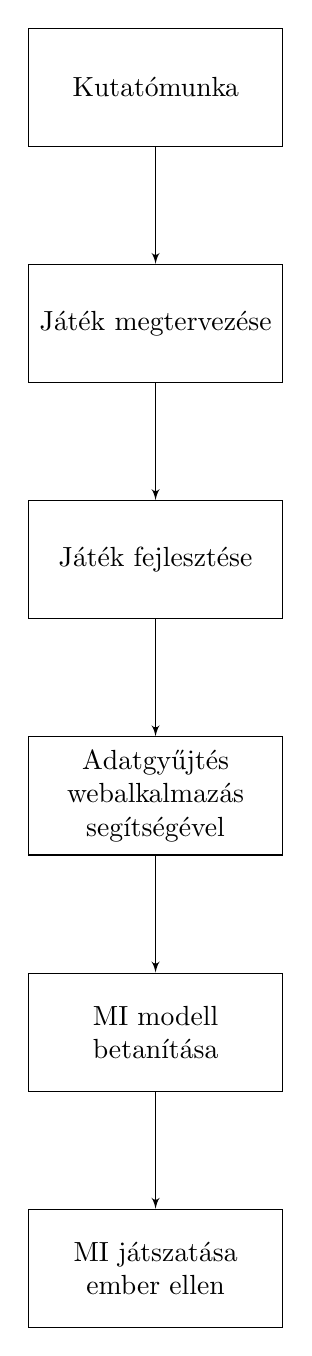
\begin{tikzpicture}[>=latex',node distance=2cm,auto]
        % Define block styles
        \tikzstyle{block} = [rectangle, draw, text width=3cm, text centered, minimum height=1.5cm ]
        \tikzstyle{line} = [draw, -latex']

        % Nodes
        \node [block] (kutatomunka) {Kutatómunka};
        \node [block, below of=kutatomunka, node distance=3cm] (tervezes) {Játék megtervezése};
        \node [block, below of=tervezes, node distance=3cm] (jatek_megirasa) {Játék fejlesztése};
        \node [block, below of=jatek_megirasa, node distance=3cm] (adatgyujtes) {Adatgyűjtés webalkalmazás segítségével};
        \node [block, below of=adatgyujtes, node distance=3cm] (MI) {MI modell betanítása};
        \node [block, below of=MI, node distance=3cm] (MI_ember) {MI játszatása ember ellen};

        % \node [block, right of=section1, node distance=4cm] (subsection1) {Subsection 1};
        % \node [block, right of=section2, node distance=4cm] (subsection2) {Subsection 2};

        % Arrows
        \path [line] (kutatomunka) -- (tervezes);
        \path [line] (tervezes) -- (jatek_megirasa);
        \path [line] (jatek_megirasa) -- (adatgyujtes);
        \path [line] (adatgyujtes) -- (MI); 
        \path [line] (MI) -- (MI_ember);

    \end{tikzpicture}
    \caption{A projekt folyamatábrája}
    \label{fig:folyamat_diagram}
\end{figure}

\subsection{Kutatómunka}
A kutatómunka során elsősorban azt vizsgáltam, hogy melyik tanító algoritmussal érhetem el a kívánt eredményt. Különböző irodalmakat tanulmányoztam, valamint áttekintettem mások munkáit a témában. A kutatómunka végeztével összegeztem a talált eredményeket.

\subsection{Játék megtervezése}
A kutatómunka után el kellett döntenem, hogy milyen játékot fejlesztek, amely elég bonyolult ahhoz, hogy kihívást jelentsen a játékosok számára, ugyanakkor elég egyszerű ahhoz, hogy az MI betanítása belátható időn belül megtörténjen. Ezen a ponton meg kellett azt is határoznom, hogy milyen technológiát alkalmazok, valamint hogy mely területekre összpontosítok a fejlesztés folyamán. A játék elkészítéséhez a Godot Enginen-t választottam.

\subsection{Játék fejlesztése}
A megfelelő tervezés után elkészítettem a választott fejlesztői környezetben a játékot. A fejlesztés során két fontos szempontot tartottam szem előtt: a játékot lehetővé kell tenni hogy játszható legyen mind HTML5 (Hypertext Markup Language 5), mind asztali számítógépen egyaránt. Biztosítanom kell, hogy az MI képes legyen kezelni a játékot csupán a játék metainformációinak ismeretében.

\subsection{Adatgyűjtés webalkalmazás segítségével}
Miután elkészült a játék, különböző korosztály tagjait kértem meg, hogy játszanak annak érdekében, hogy elegendő adatom legyen az MI betanításához. Ezt a legkönnyebben úgy tudtam elérni, ha a játékot egy erre alkalmas webes felületre kiraktam, és egy webapplikáció segítségével, folyamatosan gyűjtöttem be az adatokat. 

\subsection{MI betanítása és összekötése a játékkal}
A gyűjtött adatokat felhasználva betanítottam az MI-t egy tanító algoritmus segítségével.

A játékhoz létrehoztam egy interfészt, amely lehetővé tette az MI számára, hogy játszhasson vele. Miután ez sikeresen működött, lehetőséget teremtettem arra is, hogy az emberi játékos a gép ellen is játszhassa a játékot.